\documentclass[11pt]{article}

\usepackage{fullpage,fourier,amsmath,amssymb}
\usepackage{listings,color,url,hyperref}
\usepackage{mdframed}
\usepackage{epigraph}
\usepackage{blkarray}
\usepackage[x11names]{xcolor}

\usepackage{fancyhdr}
\pagestyle{fancy}
\fancyhf{}

\fancypagestyle{plain}{%
  \fancyhf{}
  \renewcommand{\headrulewidth}{0pt}
  \renewcommand{\footrulewidth}{0pt}
  \lfoot{\textcopyright{} 2021 Darrell Long}
  \rfoot{\thepage}
}

\pagestyle{plain}

\definecolor{codegreen}{rgb}{0,0.5,0}
\definecolor{codegray}{rgb}{0.5,0.5,0.5}
\definecolor{codepurple}{rgb}{0.58,0,0.82}

\lstloadlanguages{C,make,python,fortran}

\lstdefinestyle{c99}{
    morekeywords={bool, uint8_t, uint16_t, uint32_t, uint64_t, int8_t, int16_t, int32_t, int64_t},
    commentstyle=\color{codegreen},
    keywordstyle=\color{magenta},
    numberstyle=\tiny\color{codegray},
    identifierstyle=\color{blue},
    stringstyle=\color{codepurple},
    basicstyle=\ttfamily,
    breakatwhitespace=false,
    breaklines=true,
    captionpos=b,
    keepspaces=true,
    numbers=left,
    numbersep=5pt,
    showspaces=false,
    showstringspaces=false,
    showtabs=false,
    tabsize=4
}


\title{Assignment 4 \\ The Circumnavigations of Denver Long \\ \bigskip
\centerline{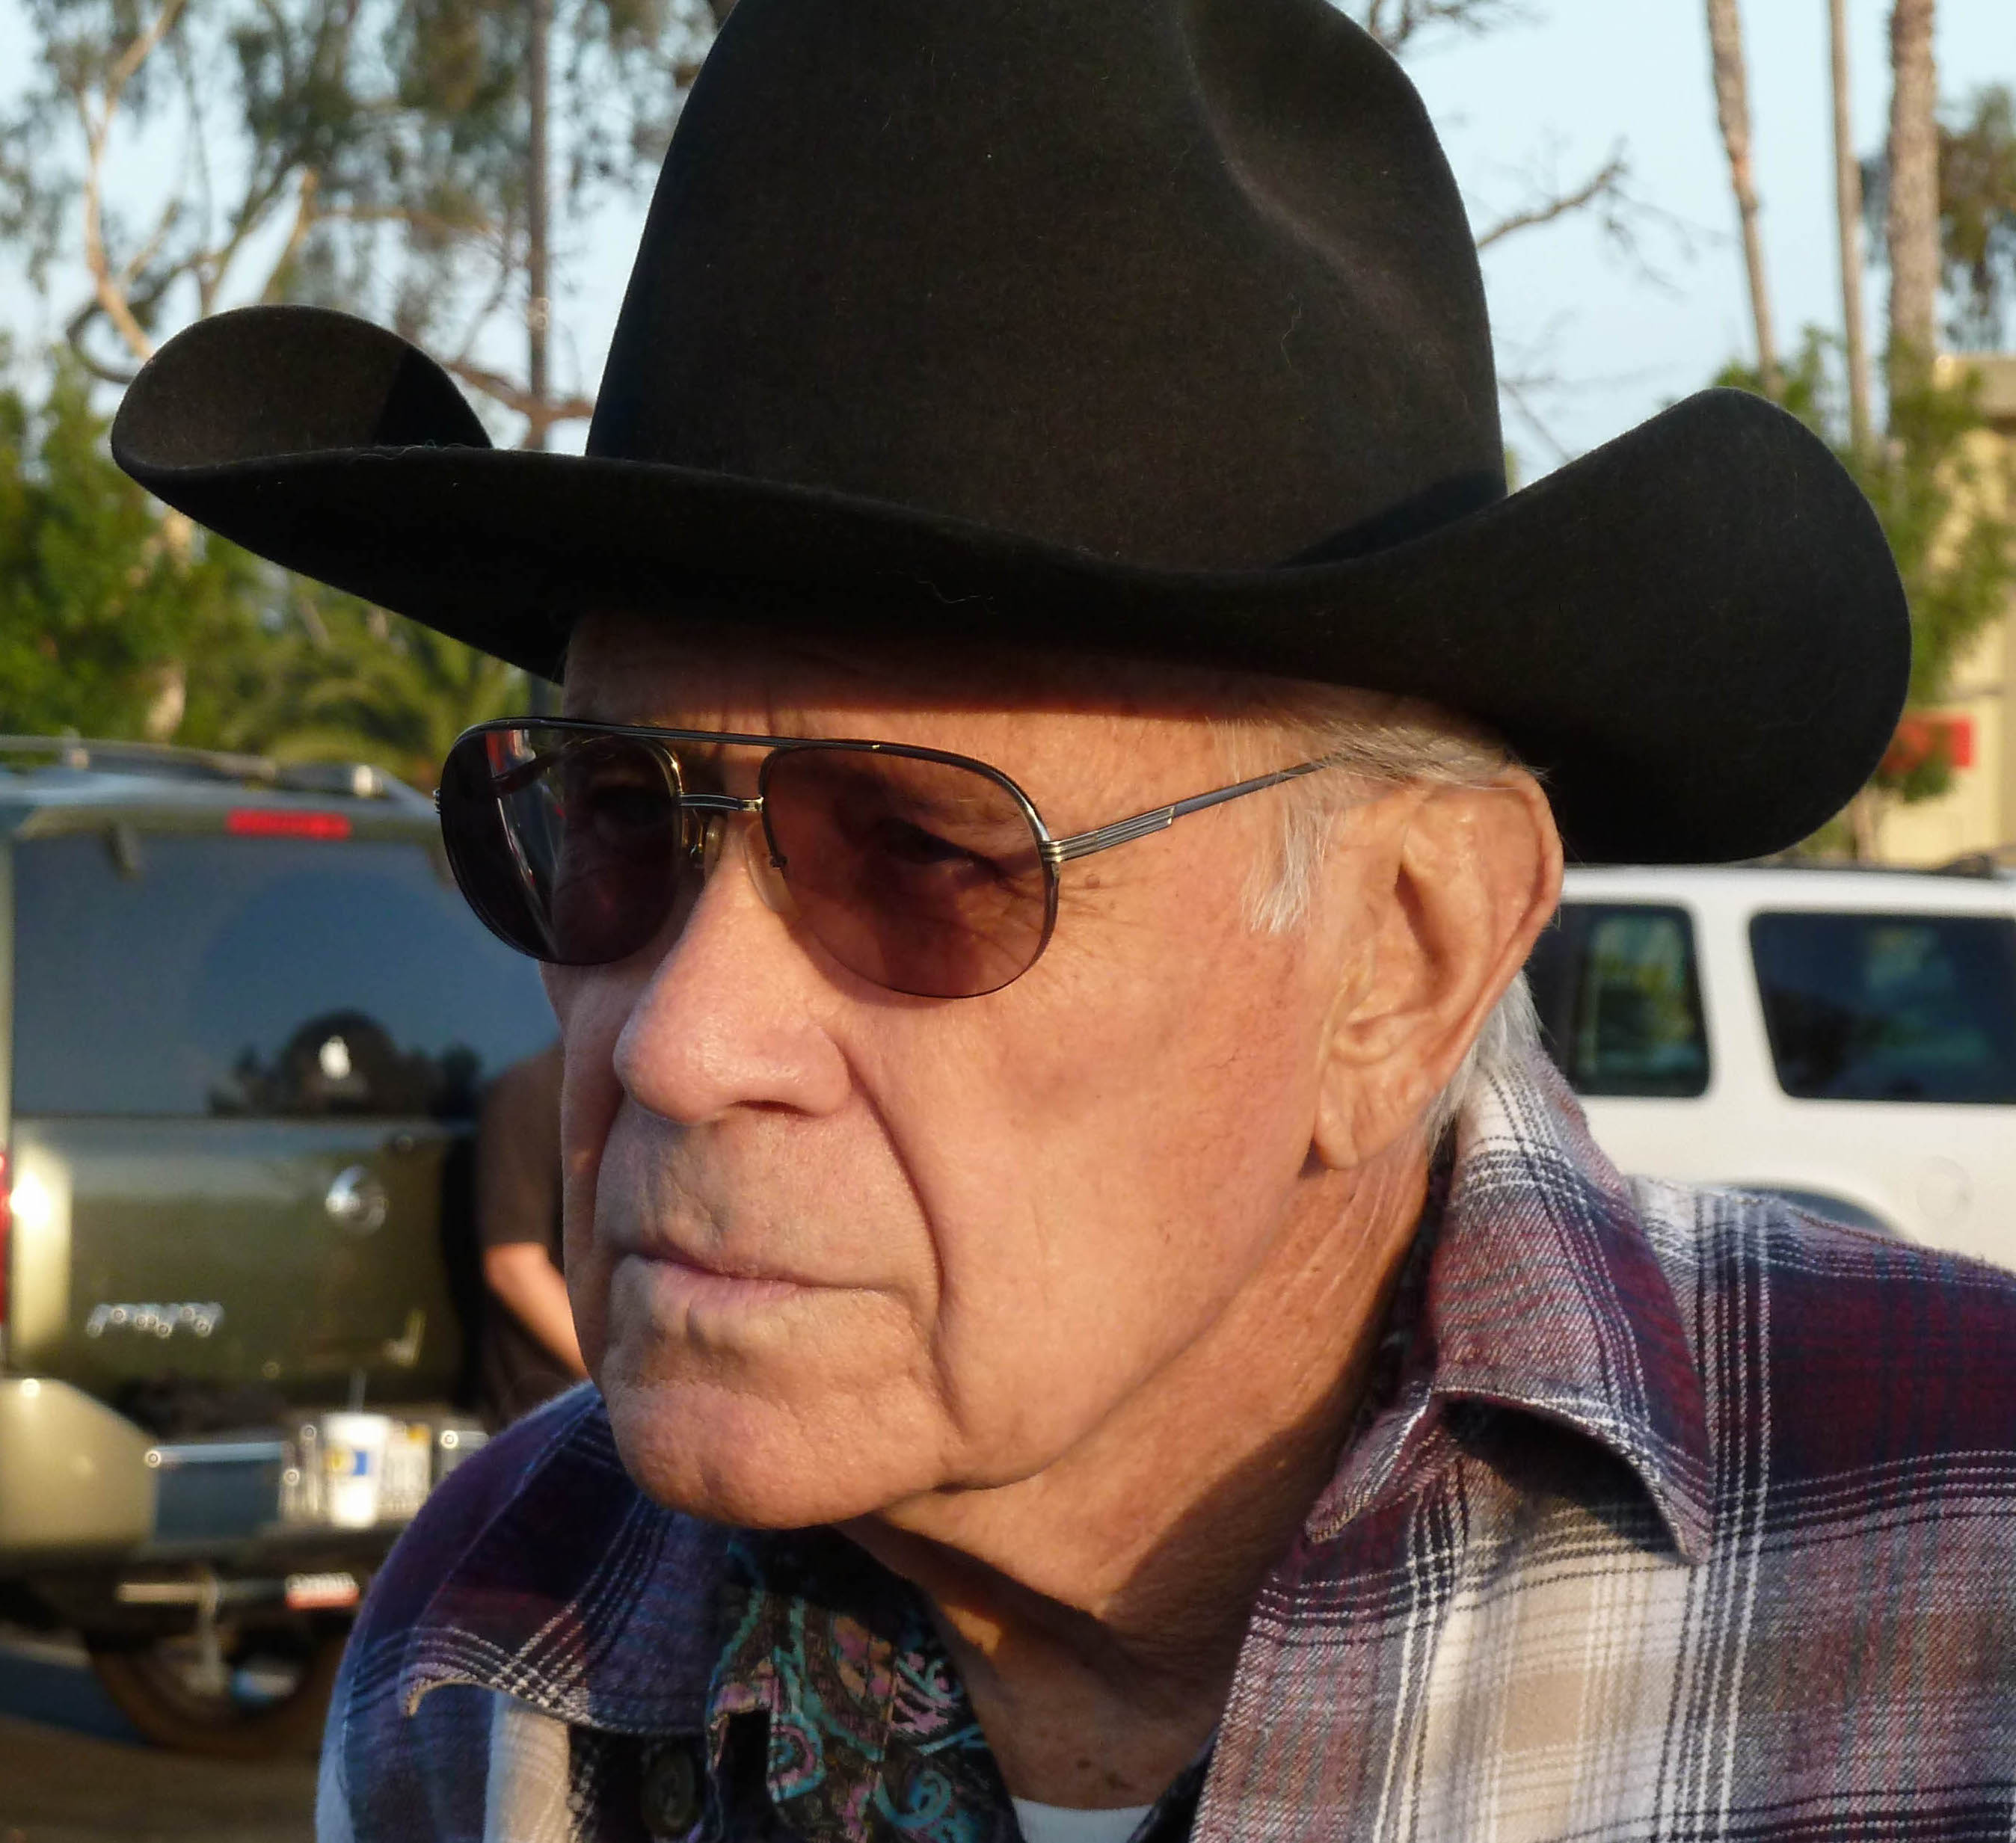
\includegraphics[width=0.3\textwidth]{images/dl.jpg}}}
\author{Prof. Darrell Long \\ CSE 13S -- Spring 2021}
\date{Due: May 2$^\text{nd}$ at 11:59\,pm}

\begin{document}

\maketitle

\section{Introduction}

\epigraphwidth=0.65\textwidth
\epigraph{\emph{I wonder why it is that when I plan a route too
    carefully, it goes to pieces, whereas if I blunder along in blissful
    ignorance aimed in a fancied direction I get through with no
    trouble.}}{---John Steinbeck, \emph{Travels with Charley: In Search
    of Amerca}}

Denver Long decides to augment his income during his retirement
years by selling the fine products produced by the Shinola Corporation.
He enjoys driving his Lincoln, and so it's the life of a traveling
salesman for him. Having accidentally taken a wrong turn near Chula
Vista and winding up in Mexico, he asks his son to have his class create
a computer program that will provide an optimal route to all the cities
along his route and then return him to his home in scenic Clearlake.

\section{Directed Graphs}

A graph is a data structure $G = \langle V, E \rangle$ where $V = \{
v_0, \ldots, v_n \}$ is the set of vertices (or nodes) and $E = \left \{
\langle v_i,v_j \rangle, \ldots \right \}$ is the set of edges that connect the
vertices. For example, you might have a set of cities $V = \{ \text{El
Cajon}, \text{La Mesa}, \text{San Diego}, \ldots, \text{La Jolla} \}$ as
the vertices and write ``El Cajon'' $\rightarrow$ ``Lakeside'' to
indicate that there is a path (Los Coches Road) from El Cajon to
Lakeside. If there is a path from El Cajon to Lakeside, as well as a
path from Lakeside to El Cajon, then the edge connecting El Cajon and
Lakeside is \emph{undirected}.

Such a simple graph representation simply tells you how vertices are
connected and provides the idea of one-way roads. But it really does not
help Denver, since it does not provide any notion of distance. We solve
this problem by associating a weight with each edge and so we might
write ``Santee $\rightarrow$ El Cajon, 2'' to indicate that there is a
path of two miles long from Santee to El Cajon. Given a set of edges
and weights, then we can then find the shortest path from any vertex to
any other vertex (the answer may be that there is no such path). There are
elegant (and quick) algorithms for computing the shortest path, but
that is not exactly what we want to do.  We want to find a path through
all of the vertices, visiting each \emph{exactly once}, such that there
is a direct (single step) connection from the last vertex to the first.
This is called a \emph{Hamiltonian path}. This will address Denver's
need to get home, but won't necessarily be the shortest such path. So,
we need to go through every possible Hamiltonian path given the list of
cities Denver is traveling through and pick the shortest path. Note: if
you find yourself on a path that is longer than the current best found
Hamiltonian path, then you can preemptively reject your current path.

\section{Representing Graphs}

\epigraphwidth=0.65\textwidth
\epigraph{\emph{Nothing can be more limiting to the imagination than
only writing about what you know.}}{---John W.\ Gardner}

Perhaps the simplest way to represent a graph is with an \emph{adjacency
matrix}. Consider an $n \times n$ adjacency matrix $M$, where $n$ is the
number of vertices in the graph. If $M_{i,j} = k$, where $1 \le i \le j
\le n$, then we say that there exists a \emph{directed edge} from vertex
$i$ to vertex $j$ with weight $k$. Traveling through wormholes is
considered hazardous, so any valid edge weight $k$ must be non-zero and
positive.

\begin{center}
\begin{blockarray}{ccccccccc}
 & 0 & 1 & 2 & 3 & 4 & 5 & $\dotsi$ & 25\\
\begin{block}{c[>{\medspace}cccccccc<{\medspace}]}
    0 & 0 & 10 & 0 & 0 & 0 & 0 & 0 & 0 \\
    1 & 0 & 0 & 2 & 5 & 0 & 0 & 0 & 0 \\
    2 & 0 & 0 & 0 & 0 & 0 & 3 & 0 & 5 \\
    3 & 0 & 0 & 0 & 0 & 21 & 0 & 0 & 0 \\
    4 & 0 & 0 & 0 & 0 & 0 & 0 & 0 & 0 \\
    5 & 0 & 0 & 0 & 0 & 0 & 0 & 0 & 0 \\
    \smash{\vdots} & 0 & 0 & 0 & 0 & 0 & 0 & 0 & 0 \\
    25 & 0 & 0 & 0 & 0 & 0 & 0 & 0 & 0 \\
\end{block}
\end{blockarray}
\end{center}

\newcommand{\edge}[3]{\langle #1,#2,#3 \rangle}

\noindent Each edge will be represented as a triplet $\edge{i}{j}{k}$. The set of
edges in the adjacency matrix above is
\[
E = \left \{
  \edge{0}{1}{10},
  \edge{1}{2}{2},
  \edge{1}{3}{5},
  \edge{2}{5}{3},
  \edge{2}{25}{5},
  \edge{3}{4}{21}
\right \}.
\]

\noindent If the above adjacency matrix were made to be \emph{undirected}, it
would be reflected along the diagonal.

\begin{center}
\begin{blockarray}{ccccccccc}
 & 0 & 1 & 2 & 3 & 4 & 5 & $\dotsi$ & 25\\
\begin{block}{c[>{\medspace}cccccccc<{\medspace}]}
    0 & 0 & 10 & 0 & 0 & 0 & 0 & 0 & 0 \\
    1 & 10 & 0 & 2 & 5 & 0 & 0 & 0 & 0 \\
    2 & 0 & 2 & 0 & 0 & 0 & 3 & 0 & 5 \\
    3 & 0 & 5 & 0 & 0 & 21 & 0 & 0 & 0 \\
    4 & 0 & 0 & 0 & 21 & 0 & 0 & 0 & 0 \\
    5 & 0 & 0 & 3 & 0 & 0 & 0 & 0 & 0 \\
    \smash{\vdots} & 0 & 0 & 0 & 0 & 0 & 0 & 0 & 0 \\
    25 & 0 & 0 & 5 & 0 & 0 & 0 & 0 & 0 \\
\end{block}
\end{blockarray}
\end{center}

\noindent We will create a graph ADT based on this \texttt{struct} definition:

\begin{codelisting}{}
struct Graph {
  uint32_t vertices;                   // Number of vertices.
  bool undirected;                     // Undirected graph?
  bool visited[VERTICES];              // Where have we gone?
  uint32_t matrix[VERTICES][VERTICES]; // Adjacency matrix.
};
\end{codelisting}

We elect to use an adjacency matrix with set maximum dimensions. This is
both to simplify the abstraction and also due to the computational
complexity of solving the Traveling Salesman Problem (TSP) with
depth-first search (DFS), which is discussed in \S 5. The
\texttt{VERTICES} macro will be defined and supplied to you in
\texttt{vertices.h}. In this header file, there is another macro
\texttt{START\_VERTEX} which defines the origin vertex of the shortest
Hamiltonian path we will be searching for.  \textcolor{red}{You may not
modify this file.} The \texttt{struct} definition of a graph \emph{must}
go in \texttt{graph.c}. The following subsections define the interface
for the graph ADT.

\begin{codelisting}{\texttt{vertices.h}}
#ifndef __VERTICES_H__
#define __VERTICES_H__

#define START_VERTEX 0   // Starting (origin) vertex.
#define VERTICES     26  // Maximum vertices in graph.

#endif
\end{codelisting}

\subsection{\texttt{Graph *graph\_create(uint32\_t vertices, bool undirected)}}

The constructor for a graph. It is through this constructor in which a
graph can be specified to be undirected. Make sure each cell of the
adjacency matrix, \texttt{matrix}, is set to zero. Also make sure that
each index of the \texttt{visited} array is initialized as
\texttt{false} to reflect that no vertex has been visited yet. The
\texttt{vertices} field reflects the number of vertices in the graph.

\subsection{\texttt{void graph\_delete(Graph **G)}}

The destructor for a graph. Remember to set the pointer \texttt{G} to
\texttt{NULL}.

\subsection{\texttt{uint32\_t graph\_vertices(Graph *G)}}

Return the number of vertices in the graph.

\subsection{\texttt{bool graph\_add\_edge(Graph *G, uint32\_t i,
uint32\_t j, uint32\_t k)}}

Adds an edge of weight \texttt{k} from vertex \texttt{i} to vertex
\texttt{j}. If the graph is undirected, add an edge, also with weight
\texttt{k} from \texttt{j} to \texttt{i}. Return \texttt{true} if both
vertices are within bounds and the edge(s) are successfully added and
\texttt{false} otherwise.

\subsection{\texttt{bool graph\_has\_edge(Graph *G, uint32\_t i,
uint32\_t j)}}

Return \texttt{true} if vertices \texttt{i} and \texttt{j} are within
bounds and there exists an edge from \texttt{i} to \texttt{j}. Remember:
an edge exists if it has a non-zero, positive weight. Return
\texttt{false} otherwise.

\subsection{\texttt{uint32\_t graph\_edge\_weight(Graph *G, uint32\_t i,
uint32\_t j)}}

Return the weight of the edge from vertex \texttt{i} to vertex
\texttt{j}. If either \texttt{i} or \texttt{j} aren't within bounds, or
if an edge doesn't exist, return 0.

\subsection{\texttt{bool graph\_visited(Graph *G, uint32\_t v)}}

Return \texttt{true} if vertex \texttt{v} has been visited and
\texttt{false} otherwise.

\subsection{\texttt{void graph\_mark\_visited(Graph *G, uint32\_t v)}}

If vertex \texttt{v} is within bounds, mark \texttt{v} as visited.

\subsection{\texttt{void graph\_mark\_unvisited(Graph *G, uint32\_t v)}}

If vertex \texttt{v} is within bounds, mark \texttt{v} as unvisited.

\subsection{\texttt{void graph\_print(Graph *G)}}

A debug function you will want to write to make sure your graph ADT
works as expected.

\section{Depth-first Search}

\epigraphwidth=0.65\textwidth \epigraph{\emph{Again it might have been
the American tendency in travel. One goes, not so much to see but to
tell afterward.}}{---John Steinbeck, \emph{Travels with Charley: In
Search of Amerca}}

We need a methodical procedure for searching through the graph. Once we
have examined a vertex, we do not want to do so again---we don't want
Denver going through cities where he has already been (he has been known
to wear out his welcome: charming women and fighting men).

Depth-first search (DFS) first marks the vertex $v$ as having been visited,
then it iterates through all of the edges $\langle v, w \rangle$,
recursively calling itself starting at $w$ if $w$ has not already been
visited.

\begin{codelisting}{}
procedure DFS(G,v):
    label v as visited
    for all edges from v to w in G.adjacentEdges(v) do
       if vertex w is not labeled as visited then
          recursively call DFS(G,w)
    label v as unvisited
\end{codelisting}

Finding a Hamiltonian path then reduces to:
\begin{enumerate}
\item
Using DFS to find paths that pass through all vertices, and
\item
There is an edge from the last vertex to the first. The solutions to the
Traveling Salesman Problem are then the shortest found Hamiltonian
paths.
\end{enumerate}

\section{Computational Complexity}

\epigraphwidth=0.65\textwidth \epigraph{\emph{Many a trip continues long
    after movement in time and space have ceased. I remember a man in
    Salinas who in his middle years traveled to Honolulu and back, and
    that journey continued for the rest of his life. We could watch him
    in his rocking chair on his front porch, his eyes squinted,
    half-closed, endlessly traveling to Honolulu.}}{---John Steinbeck,
    \emph{Travels with Charley: In Search of Amerca}}

How long will this take?
The answer is, it will take a very long time if there are a large number
of vertices. The running time of the simplest algorithm is
$\operatorname{O}(n!)$ and there is no known algorithm that runs in less
than $\operatorname{O}(2^n)$ time.  In fact, the TSP has been shown to
be NP-hard, which means that it is as difficult as any problem in the
class NP (you will learn more about this in CSE\,104: Computability and
Computational Complexity).  Basically, it means that it can be solved in
polynomial time if you have a magical computer that at each if-statement
is takes both branches every time (creating a copy of the computer for
each such branch).

\section{Representing Paths}

\epigraphwidth=0.65\textwidth \epigraph{\emph{We find after years of
struggle that we do not take a trip; a trip takes us.} }{---John
Steinbeck, \emph{Travels with Charley: In Search of Amerca}}

Given that vertices are added to and removed from the traveled path in a
stack-like manner, we decide to abstract a path as follows:

\begin{codelisting}{}
struct Path {
  Stack *vertices; // The vertices comprising the path.
  uint32_t length; // The total length of the path.
};
\end{codelisting}


The following subsections define for the interface for the path ADT.

\subsection{\texttt{Path *path\_create(void)}}

The constructor for a path. Set \texttt{vertices} as a freshly created
stack that can hold up to \texttt{VERTICES} number of vertices.
Initialize \texttt{length} to be 0. The \texttt{length} field will track
the length of the path. In other words, it holds the sum of the edge
weights between consecutive vertices in the \texttt{vertices} stack.

\subsection{\texttt{void path\_delete(Path **p)}}

The destructor for a path. Remember to set the pointer \texttt{p} to
\texttt{NULL}.

\subsection{\texttt{bool path\_push\_vertex(Path *p, uint32\_t v, Graph
*G)}}

Pushes vertex \texttt{v} onto path \texttt{p}. The \texttt{length} of the
path is \emph{increased} by the edge weight connecting the vertex at the top of
the stack and \texttt{v}. Return \texttt{true} if the vertex was
successfully pushed and \texttt{false} otherwise.

\subsection{\texttt{bool path\_pop\_vertex(Path *p, uint32\_t *v, Graph
*G)}}

Pops the \texttt{vertices} stack, passing the popped vertex back through
the pointer \texttt{v}. The \texttt{length} of the path is
\emph{decreased} by the edge weight connecting the vertex at the top of
the stack and the popped vertex. Return \texttt{true} if the vertex was
successfully popped and \texttt{false} otherwise.

\subsection{\texttt{uint32\_t path\_vertices(Path *p)}}

Returns the number of vertices in the path.

\subsection{\texttt{uint32\_t path\_length(Path *p)}}

Returns the length of the path.

\subsection{\texttt{void path\_copy(Path *dst, Path *src)}}

Assuming that the destination path \texttt{dst} is properly initialized,
makes \texttt{dst} a copy of the source path \texttt{src}. This will
require making a copy of the \texttt{vertices} stack as well as the
\texttt{length} of the source path.

\subsection{\texttt{void path\_print(Path *p, FILE *outfile, char
*cities[])}}

Prints out a path to \texttt{outfile} using \texttt{fprintf()}. Requires
a call to \texttt{stack\_print()}, as defined in \S 7.10, in order to
print out the contents of the \texttt{vertices} stack.

\section{Stacks, Revisited}

\epigraphwidth=0.55\textwidth \epigraph{\emph{If you have some respect
for people as they are, you can be more effective in helping them to
become better than they are.}}{---John W.\ Gardner}

You will use the stack that you implemented for assignment 3 with slight
modifications. If there were any problems with your stack for that
assignment, make sure to fix them for this assignment. Here is the
modified stack interface for this assignment.

\begin{codelisting}{}
struct Stack {
    uint32_t top;
    uint32_t capacity;
    uint32_t *items;
};
\end{codelisting}

\subsection{\texttt{Stack *stack\_create(uint32\_t capacity)}}

The constructor function for a \texttt{Stack}. The \texttt{top} of a
stack should be initialized to 0. The capacity of a stack is set to the
specified capacity. The specified capacity also indicates the number of
items to allocate memory for, the items in which are held in the
dynamically allocated array \texttt{items}.

\subsection{\texttt{void stack\_delete(Stack **s)}}

The destructor function for a stack. Remember to set the pointer
\texttt{s} to \texttt{NULL}.

\subsection{\texttt{bool stack\_empty(Stack *s)}}

Return \texttt{true} if the stack is empty and \texttt{false} otherwise.

\subsection{\texttt{bool stack\_full(Stack *s)}}

Return \texttt{true} if the stack is full and \texttt{false} otherwise.

\subsection{\texttt{uint32\_t stack\_size(Stack *s)}}

Return the number of items in the stack.

\subsection{\texttt{bool stack\_push(Stack *s, uint32\_t x)}}

If the stack is full prior to pushing the item \texttt{x}, return
\texttt{false} to indicate failure.  Otherwise, push the item and return
\texttt{true} to indicate success.

\subsection{\texttt{bool stack\_peek(Stack *s, uint32\_t *x)}}

Peeking into a stack is synonymous with querying a stack about the
element at the top of the stack.  If the stack is empty prior to peeking
into it, return \texttt{false} to indicate failure.

\subsection{\texttt{bool stack\_pop(Stack *s, uint32\_t *x)}}

If the stack is empty prior to popping it, return \texttt{false} to
indicate failure. Otherwise, pop the item, set the value in the memory
\texttt{x} is pointing to as the popped item, and return \texttt{true}
to indicate success.

\subsection{\texttt{void stack\_copy(Stack *dst, Stack *src)}}

Assuming that the destination stack \texttt{dst} is properly initialized,
make \texttt{dst} a copy of the source stack \texttt{src}. This means
making the \emph{contents} of \texttt{dst->items} the same as
\texttt{src->items}. The top of \texttt{dst} should also match the top
of \texttt{src}.

\subsection{\texttt{void stack\_print(Stack *s, FILE *outfile, char
*cities[])}}

Prints out the contents of the stack to \texttt{outfile} using
\texttt{fprintf()}. Working through each vertex in the stack starting
from the \emph{bottom}, print out the name of the city each vertex
corresponds to. This function will be given to aid you.

\begin{codelisting}{}
void stack_print(Stack *s, FILE *outfile, char *cities[]) {
    for (uint32_t i = 0; i < s->top; i += 1) {
        fprintf(outfile, "%s", cities[s->items[i]]);
        if (i + 1 != s->top) {
            fprintf(outfile, " -> ");
        }
    }
    fprintf(outfile, "\n");
}
\end{codelisting}

\section{Command-line Options}

\epigraphwidth=0.65\textwidth
\epigraph{\emph{Attitude is a choice. Happiness is a choice. Optimism is
a choice. Kindness is a choice. Giving is a choice. Respect is a choice.
Whatever choice you make makes you. Choose wisely.}}{---Roy T.\ Bennett,
\emph{The Light in the Heart}}

Your program must support any combination of the following command-line
options.

\begin{itemize}
  \item \textbf{\texttt{-h}}\,: Prints out a help message describing the purpose
    of the graph and the command-line options it accepts, exiting the
    program afterwards. Refer to the reference program in the resources
    repo for an idea of what to print.
  \item \textbf{\texttt{-v}}\,: Enables verbose printing. If enabled,
    the program prints out \emph{all} Hamiltonian paths found as well as
    the total number of recursive calls to \texttt{dfs()}.
  \item \textbf{\texttt{-u}}\,: Specifies the graph to be undirected.
  \item \textbf{\texttt{-i infile}}\,: Specify the input file path
    containing the cities and edges of a graph. If not specified, the
    default input should be set as \texttt{stdin}.
  \item \textbf{\texttt{-o outfile}}\,: Specify the output file path to
    print to. If not specified, the default output should be set as
    \texttt{stdout}.
\end{itemize}

\section{Reading An Input Graph}

\epigraphwidth=0.5\textwidth
\epigraph{\emph{It behooves a man who
wants to see wonders sometimes to go out of his way.}}{---John
Mandeville, \emph{The Travels of Sir John Mandeville}}

We will be storing graphs in specially formatted files. Here is an
example:

\begin{lstlisting}[style=bashstyle]
  $ cat mythical.graph
  4
  Asgard
  Elysium
  Olympus
  Shangri-La
  0 3 5
  3 2 4
  2 1 10
  1 0 2
\end{lstlisting}

The first line of a graph file is the number of vertices, or cities, in
the graph. Assuming $n$ is the number of vertices, the next $n$ lines
of the file are the names of the cities. Each line after that is an
edge. It is to be scanned in as a triplet $\edge{i}{j}{k}$ and
interpreted as an edge from vertex $i$ to vertex $j$ with weight $k$.

\section{Specifics}

\epigraphwidth=0.5\textwidth
\epigraph{\emph{The gladdest moment in
human life, methinks, is a departure into unknown lands.}}{---Sir
Richard Burton}

Here are the specifics for your program implementation.

\begin{enumerate}
  \item Parse command-line options with looped calls to
    \texttt{getopt()}. This should be familiar from assignments 2 and 3.
  \item Scan in the first line from the input. This will be the
    number of vertices, or cities, that will be in the graph. Print an
    error if the number specified is greater than \texttt{VERTICES}, the
    macro defined in \texttt{vertices.h}.
  \item Assuming the number of specified vertices is $n$, read the next
    $n$ lines from the input using \texttt{fgets()}. Each line is the
    name of a city. Save the name of each city to an array. You will
    want to either make use of \texttt{strdup()} from
    \texttt{<string.h>} or implement your own \texttt{strdup()}
    function. If the line is malformed, print an error
    and exit the program. Note: using \texttt{fgets()} will leave in the
    newline character at the end, so you will manually have to change it
    to the null character to remove it.
  \item Create a new graph $G$, making it undirected if specified.
  \item Scan the input line by line using \texttt{fscanf()} until the
    end-of-file is reached.  Add each edge to $G$. If the line is
    malformed, print an error and exit the program.
  \item Create two paths. One will be for tracking the current traveled path and
    the other for tracking the shortest found path.
  \item Starting from the origin vertex, defined by the macro
    \texttt{START\_VERTEX} in \texttt{vertices.h}, perform a depth-first
    search on $G$ to find the shortest Hamiltonian path. Here is an
    example function prototype that you may use as the recursive
    depth-first function:

\begin{codelisting}{}
void dfs(Graph *G, uint32_t v, Path *curr, Path *shortest, char *cities[], FILE *outfile);
\end{codelisting}

    The parameter \texttt{v} is the vertex that you are currently on.
    The currently traversed path is maintained with \texttt{curr}. The
    shortest found path is tracked with \texttt{shortest}. The array of
    city names is \texttt{cities}. Finally, \texttt{outfile} is the
    output to print to.

  \item After the search, print out the length of the shortest path
    found, the path itself (remember to return back to the origin), and
    the number of calls to \texttt{dfs()}.

\begin{lstlisting}[style=bashstyle]
  $ ./tsp < mythical.graph
  Path length: 21
  Path: Asgard -> Shangri-La -> Olympus -> Elysium -> Asgard
  Total recursive calls: 4
\end{lstlisting}

    If the verbose command-line option was enabled, print out \emph{all}
    the Hamiltonian paths that were found as well. It is recommended
    that you print out the paths as you find them.

\begin{lstlisting}[style=bashstyle]
  $ ./tsp -v < ucsc.graph
  Path length: 7
  Path: Cowell -> Stevenson -> Merrill -> Cowell
  Path length: 6
  Path: Cowell -> Merrill -> Stevenson -> Cowell
  Path length: 6
  Path: Cowell -> Merrill -> Stevenson -> Cowell
  Total recursive calls: 5
\end{lstlisting}
\end{enumerate}

\section{Deliverables}

\epigraphwidth=0.65\textwidth \epigraph{\emph{Travel isn't always
    pretty. It isn't always comfortable. Sometimes it hurts, it even
    breaks your heart. But that's okay. The journey changes you; it
    should change you. It leaves marks on your memory, on your
consciousness, on your heart, and on your body. You take something with
you. Hopefully, you leave something good behind.}}{---Anthony Bourdain
}

\begin{enumerate}
  \item Your program, called \texttt{tsp}, \emph{must} have the
    following source and header files:
    \begin{itemize}
      \item \texttt{vertices.h} defines macros regarding vertices.
      \item \texttt{graph.h} specifies the interface to the graph ADT.
      \item \texttt{graph.c} implements the graph ADT.
      \item \texttt{stack.h} specifies the interface to the stack ADT.
      \item \texttt{stack.c} implements the stack ADT.
      \item \texttt{path.h} specifies the interface to the path ADT.
      \item \texttt{path.c} implements the path ADT.
      \item \texttt{tsp.c} contains \texttt{main()} and \emph{may}
        contain any other functions necessary to complete the
        assignment.
    \end{itemize}

You can have other source and header files, but \emph{do not try to be
overly clever}. \textbf{\textcolor{red}{You may not modify any of the supplied
header files.}}

  \item \texttt{Makefile}: This is a file that will allow the grader to
    type \texttt{make} or \texttt{make all} to compile your program.
    \begin{itemize}
      \item \texttt{CC=clang} must be specified.
      \item \texttt{CFLAGS=-Wall -Wextra -Werror -Wpedantic}
        must be included.
      \item \texttt{make} should build your program, as should
        \texttt{make all}.
      \item \texttt{make clean} must remove all files that are compiler
        generated.
      \item \texttt{make format} should format all your source code,
        including the header files.
    \end{itemize}

  \item Your code must pass \texttt{scan-build} \emph{cleanly}.

  \item \texttt{README.md}: This \emph{must} be in \emph{Markdown}.
    This must describe your program briefly, its usage, and how to build
    it using your \texttt{Makefile}.

  \item \texttt{DESIGN.pdf}: This \emph{must} be a PDF. The design
    document should contain answers to the pre-lab questions at the
    beginning and describe your design for your program with enough
    detail that a sufficiently knowledgeable programmer would be able to
    replicate your implementation. This does not mean copying your
    entire program in verbatim. You should instead describe how your
    program works with supporting pseudo-code.

\end{enumerate}

\section{Supplemental Readings}

\epigraph{\emph{One of the reasons people stop learning is that they
become less and less willing to risk failure.  you learn, the more
places you'll go.}}{---John W.\ Gardner}

\begin{itemize}
  \item \textit{The C Programming Language} by Kernighan \& Ritchie
  \begin{itemize}
    \item Chapter 4 \S 4.10
    \item Chapter 7 \S 7.4--7.8
  \end{itemize}
  \item \textit{Introduction to Algorithms} by T.\ Cormen, C.\
    Leiserson, R.\ Rivest, \& C.\ Stein
    \begin{itemize}
      \item Chapter 10 \S 10.1
      \item Chapter 35 \S 35.2
    \end{itemize}
\end{itemize}

\section{Submission}

\epigraph{\emph{A man who procrastinates in his choosing will inevitably
have his choice made for him by circumstance.}}{---Hunter S.\
Thompson, \emph{The Proud Highway}}

Refer back to \texttt{asgn0} for the steps on how to submit your
assignment through \texttt{git}. Remember: \emph{add, commit,} and
\emph{push}! \textcolor{red}{Your assignment is turned in \emph{only}
  after you have pushed \emph{and} submitted the commit ID on Canvas. If
you forget to push, you have not turned in your assignment and you will
get a \emph{zero}. ``I forgot to push'' is not a valid excuse. It is
\emph{highly} recommended to commit and push your changes \emph{often}.}

\begin{center}
  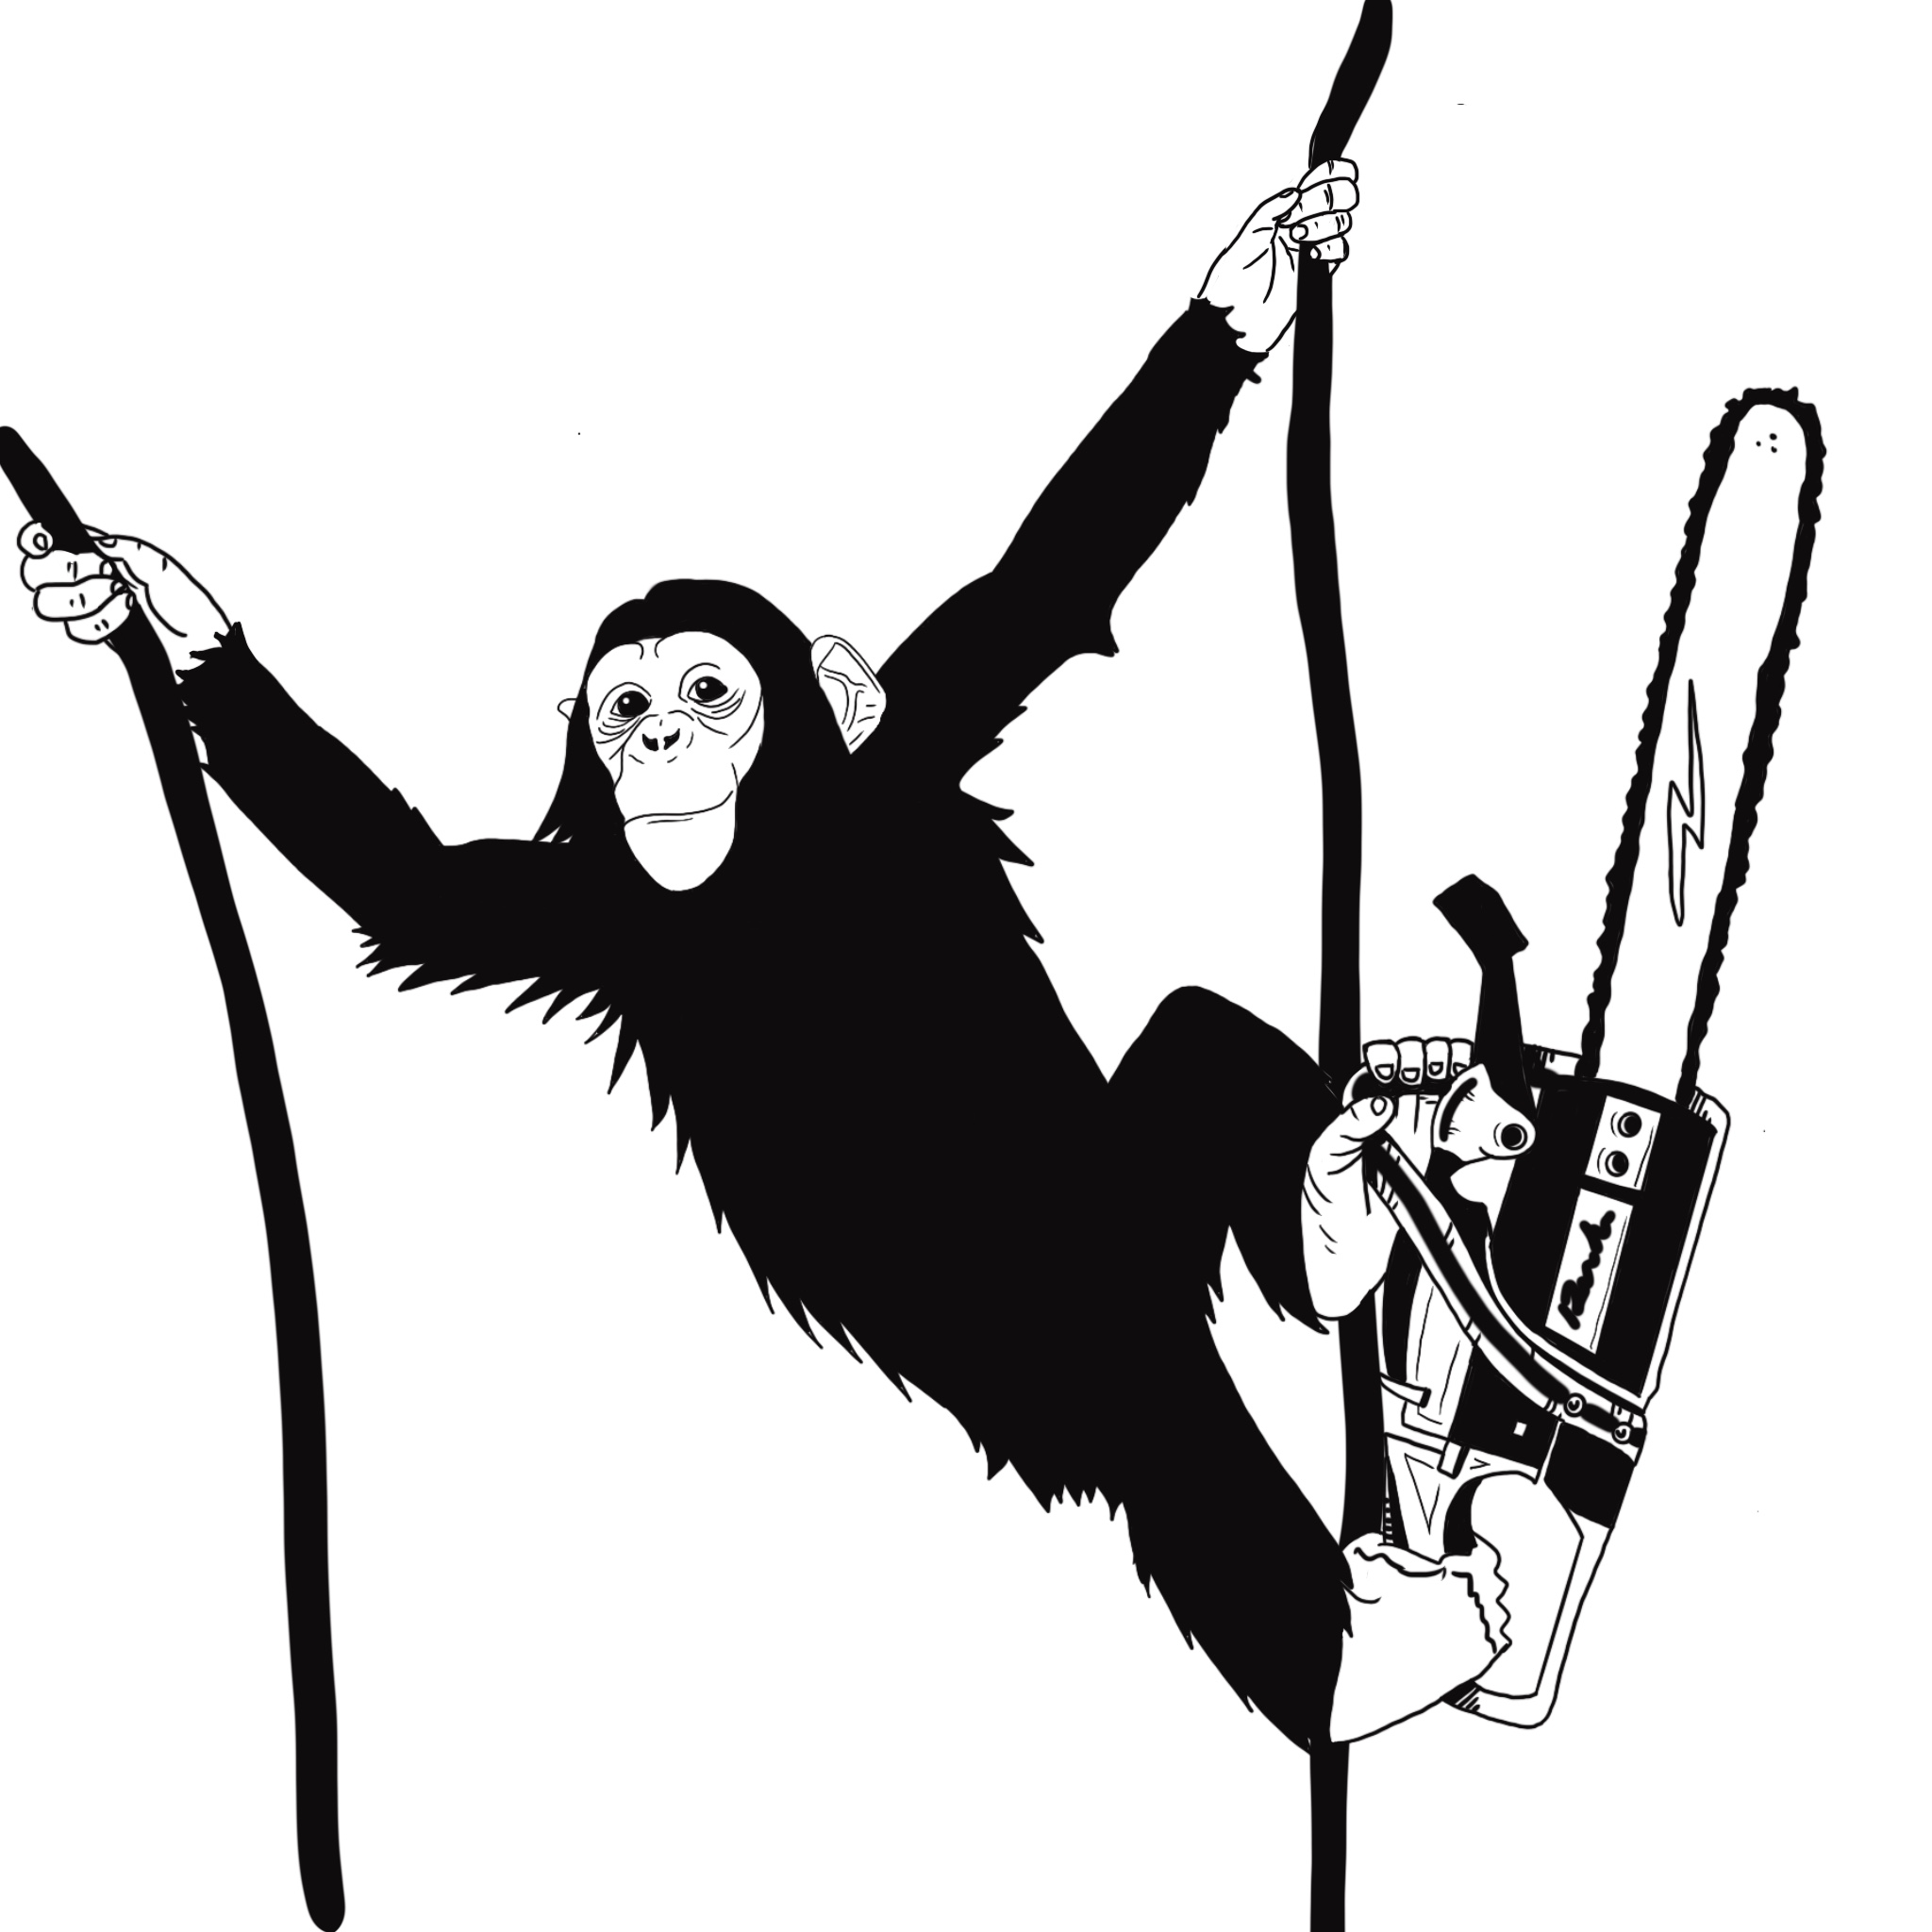
\includegraphics[width=0.45\textwidth]{../../images/monkey-chainsaw.jpg} \\
  \vspace{10pt}
  % Caesar Cipher, shift 16.
  \texttt{Fhewhqccydw yd S yi byau wylydw q cedauo q sxqydiqm.}
\end{center}

\end{document}
